\documentclass[12pt]{article}

\thispagestyle{empty}
\usepackage[scale=.95]{geometry}

\usepackage{amsmath}
\usepackage{fontspec}
\usepackage{unicode-math}
\setmainfont{TeX Gyre Bonum}
\setmathfont{TeX Gyre Bonum Math}

\usepackage{tcolorbox}
\usepackage{varwidth}

\usepackage{tikz}
\usetikzlibrary{
  matrix,
  matrix.skeleton,
  decorations.pathreplacing,
  calligraphy,
  positioning,
  arrows.meta,
  calc,
  fit,
  tikzmark
}

\usepackage{siunitx}
\usepackage{tikzpagenodes}

\ExplSyntaxOn
\cs_new_protected_nopar:Npn \circle_row:n #1
{
  \(\ang{\int_eval:n{#1}}\) \&
  \(\ang{90}\) \&
  \(\ang{\int_eval:n {90-#1}}\) \&
  \(\ang{\int_eval:n{90}}\) \&
  \(\ang{\int_eval:n{#1}}\) \&
  \(\ang{\int_eval:n {#1}}\)
}
\cs_generate_variant:Nn \circle_row:n {V}

\int_new:N \l__circle_random_a_int
\DeclareDocumentCommand \RandomCircleRow { m }
{
  \int_set:Nn \l__circle_random_a_int {\int_rand:n {90/#1-1} * #1}
  \circle_row:V \l__circle_random_a_int
}
\DeclareDocumentCommand \CircleRow {m}
{
  \circle_row:n {#1}
}

\ExplSyntaxOff

\tikzset{
  >=Latex,
  show cell/.style 2 args={
    row #1 column #2/.style={
      every node/.append style={text opacity=1}
    },
  },
  current row/.initial=1,
  step current row/.style={
    current row/.expanded={\the\numexpr\pgfkeysvalueof{/tikz/current row}+1\relax}
  },
  show cell on current row/.style={
    show cell={\pgfkeysvalueof{/tikz/current row}}{#1}
  },
  show cells/.style 2 args={
    current row=#1,
    show cell on current row/.list={#2}
  },
  show cells on next row/.style={
    step current row,
    show cell on current row/.list={#1}
  }
}

\begin{document}

\begin{center}
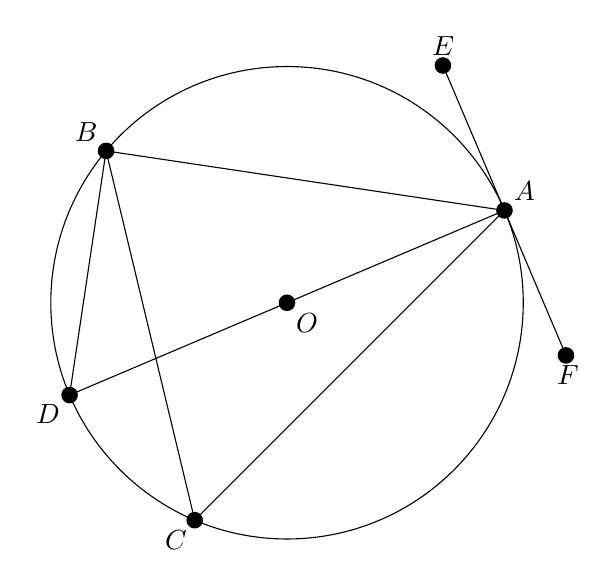
\begin{tikzpicture}
\coordinate (O) at (0,0);
\coordinate (A) at (23:3cm);
\coordinate (B) at (140:3cm);
\coordinate (C) at (-113:3cm);
\coordinate (D) at (203:3cm);
\coordinate (E) at ($(A)!2cm!-90:(O)$);
\coordinate (F) at ($(A)!2cm!90:(O)$);
\draw (0,0) circle[radius=3cm];
\draw (A) -- (B) -- (C) -- cycle;
\draw (B) -- (D) -- (A);
\draw (E) -- (F);
\foreach \k/\anch in {%
  O/below right,
  A/above right,
  B/above left,
  C/below left,
  D/below left,
  E/above,
  F/below%
} {
  \fill (\k) circle[radius=3pt];
  \node[\anch] at (\k) {\(\k\)};
}
\end{tikzpicture}
\end{center}


\begin{center}
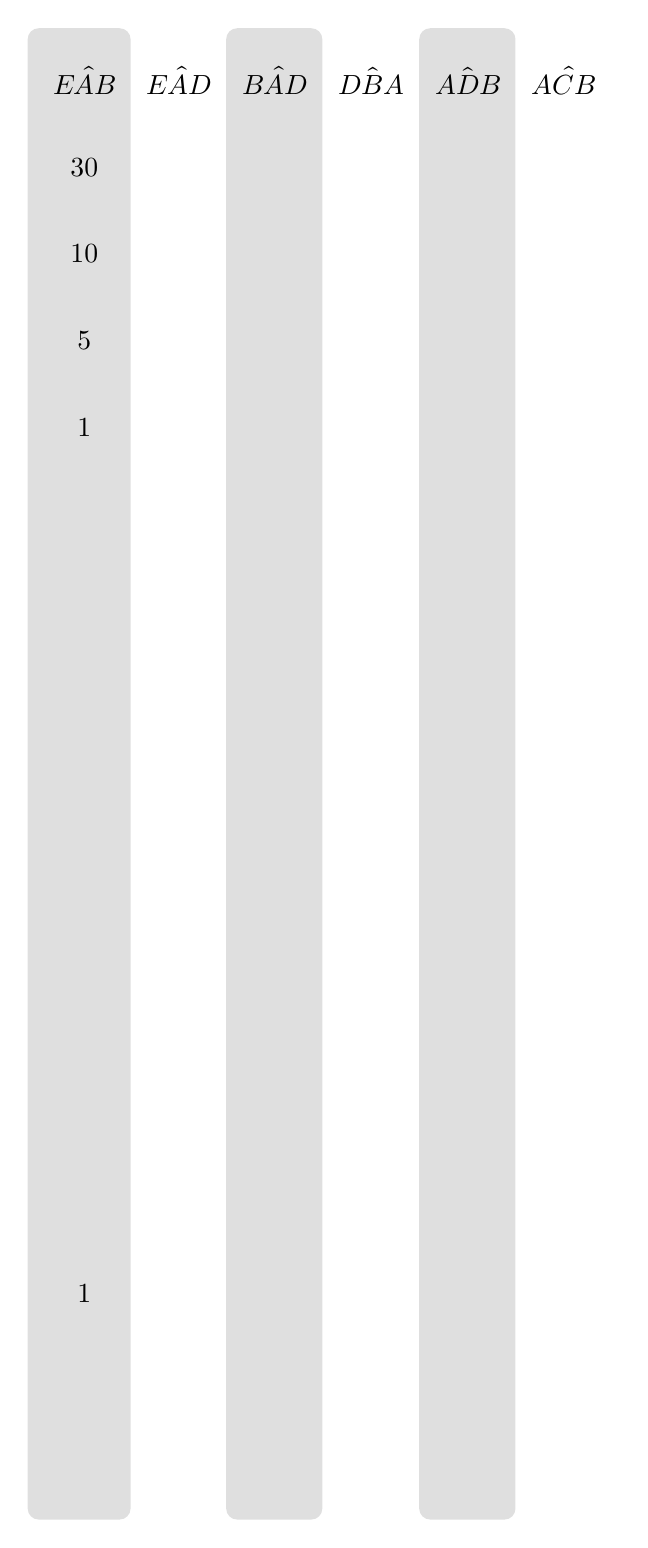
\begin{tikzpicture}
\matrix[
  matrix of nodes,
  ampersand replacement=\&,
  nodes={inner xsep=2mm, minimum width=.8cm,
    text opacity=0,
    minimum height=1.1cm},
  row 1/.style={every node/.append style={font=\bfseries,text opacity=1}},
  style odd tiling columns={fill=gray!25,rounded corners},
  %
  row 2/.style={every node/.append style={text opacity=1}},
  %
  current row=2,
  show cells on next row={1},
  show cells on next row={1},
  show cells on next row={1},
  show cells on next row={3},
  show cells on next row={3},
  show cells on next row={3},
  show cells on next row={5},
  show cells on next row={5},
  show cells on next row={5},
  show cells on next row={6},
  show cells on next row={6},
  show cells on next row={6},
  show cells on next row={1},
  show cells on next row={3},
  show cells on next row={6},
]
(m)
{
  \(E\hat{A}B\) \&
  \(E\hat{A}D\) \&
  \(B\hat{A}D\) \&
  \(D\hat{B}A\) \&
  \(A\hat{D}B\) \&
  \(A\hat{C}B\) \\
  %
  \CircleRow{30} \\
  \RandomCircleRow{10} \\
  \RandomCircleRow{5} \\
  \RandomCircleRow{1} \\
  \RandomCircleRow{10} \\
  \RandomCircleRow{5} \\
  \RandomCircleRow{1} \\
  \RandomCircleRow{10} \\
  \RandomCircleRow{5} \\
  \RandomCircleRow{1} \\
  \RandomCircleRow{10} \\
  \RandomCircleRow{5} \\
  \RandomCircleRow{1} \\
  \RandomCircleRow{1} \\
  \RandomCircleRow{1} \\
  \RandomCircleRow{1} \\
};

\end{tikzpicture}
\end{center}



\end{document}
